%%%%%%%%%%%%%%%%%%%%%%%%%%%%%%%%%%%%%%%%%
% Beamer Presentation
% LaTeX Template
% Version 1.0 (10/11/12)
%
% This template has been downloaded from:
% http://www.LaTeXTemplates.com
%
% License:
% CC BY-NC-SA 3.0 (http://creativecommons.org/licenses/by-nc-sa/3.0/)
%
%%%%%%%%%%%%%%%%%%%%%%%%%%%%%%%%%%%%%%%%%

%----------------------------------------------------------------------------------------
%	PACKAGES AND THEMES
%----------------------------------------------------------------------------------------

\documentclass{beamer}

\mode<presentation> {

% The Beamer class comes with a number of default slide themes
% which change the colors and layouts of slides. Below this is a list
% of all the themes, uncomment each in turn to see what they look like.

%\usetheme{default}
%\usetheme{AnnArbor}
%\usetheme{Antibes}
%\usetheme{Bergen}
%\usetheme{Berkeley}
%\usetheme{Berlin}
%\usetheme{Boadilla}
%\usetheme{CambridgeUS}
%\usetheme{Copenhagen}
%\usetheme{Darmstadt}
%\usetheme{Dresden}
%\usetheme{Frankfurt}
%\usetheme{Goettingen}
%\usetheme{Hannover}
%\usetheme{Ilmenau}
%\usetheme{JuanLesPins}
%\usetheme{Luebeck}
\usetheme{Madrid}
%\usetheme{Malmoe}
%\usetheme{Marburg}
%\usetheme{Montpellier}
%\usetheme{PaloAlto}
%\usetheme{Pittsburgh}
%\usetheme{Rochester}
%\usetheme{Singapore}
%\usetheme{Szeged}
%\usetheme{Warsaw}

% As well as themes, the Beamer class has a number of color themes
% for any slide theme. Uncomment each of these in turn to see how it
% changes the colors of your current slide theme.

%\usecolortheme{albatross}
%\usecolortheme{beaver}
%\usecolortheme{beetle}
%\usecolortheme{crane}
%\usecolortheme{dolphin}
%\usecolortheme{dove}
%\usecolortheme{fly}
%\usecolortheme{lily}
%\usecolortheme{orchid}
%\usecolortheme{rose}
%\usecolortheme{seagull}
%\usecolortheme{seahorse}
%\usecolortheme{whale}
%\usecolortheme{wolverine}

%\setbeamertemplate{footline} % To remove the footer line in all slides uncomment this line
%\setbeamertemplate{footline}[page number] % To replace the footer line in all slides with a simple slide count uncomment this line

%\setbeamertemplate{navigation symbols}{} % To remove the navigation symbols from the bottom of all slides uncomment this line
}

\usepackage{graphicx} % Allows including images
\usepackage{booktabs} % Allows the use of \toprule, \midrule and \bottomrule in tables
\usepackage{multirow}
\newcommand{\xmark}{\textcolor{red}{\text{\sffamily X}}}
\newcommand{\cmark}{\textcolor{green}{\checkmark}}
%----------------------------------------------------------------------------------------
%	TITLE PAGE
%----------------------------------------------------------------------------------------


\title[Group talk]{A function MRI mind-reading game}

\author{Charles Zheng and Yuval Benjamini} % Your name
\institute[Stanford] % Your institution as it will appear on the bottom of every slide, may be shorthand to save space
{Stanford University}
\date{\today} % Date, can be changed to a custom date

\begin{document}

\begin{frame}
\titlepage % Print the title page as the first slide
\end{frame}

\section{Introduction}

\frame{\sectionpage}

\begin{frame}
\frametitle{Functional MRI}
\begin{center}
\begin{tabular}{ccc}
\hline
Stimuli & & Response\\ \hline
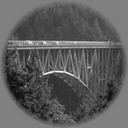
\includegraphics[scale = .52]{img1.png} & \hspace{1in} & 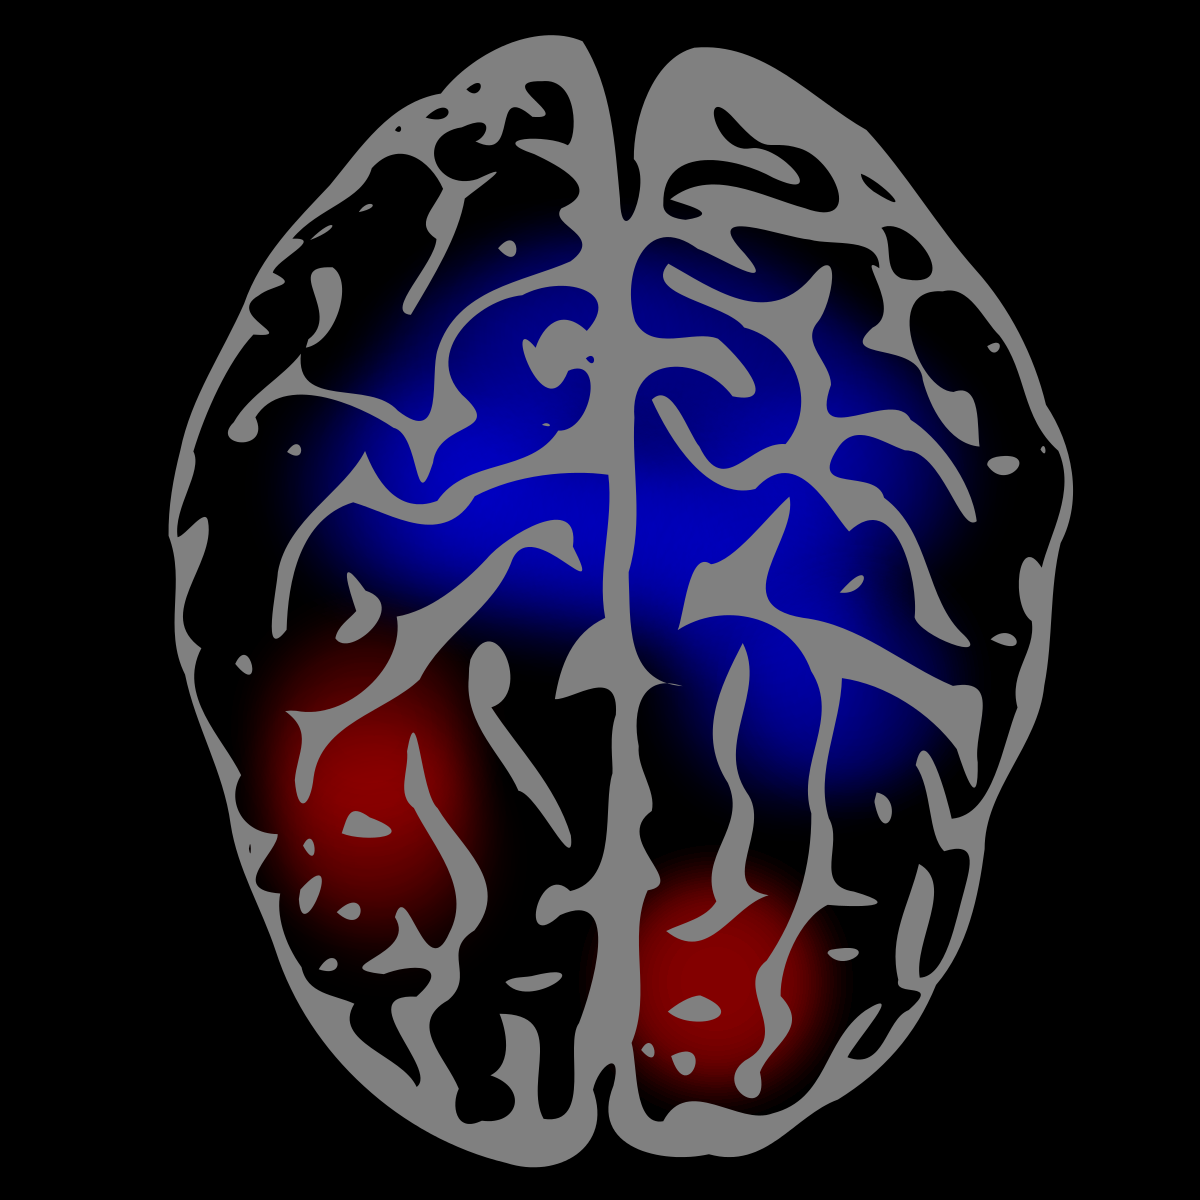
\includegraphics[scale = 0.07]{brain1.png} \\ \hline
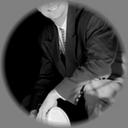
\includegraphics[scale = .52]{img2.png} & \hspace{1in} & 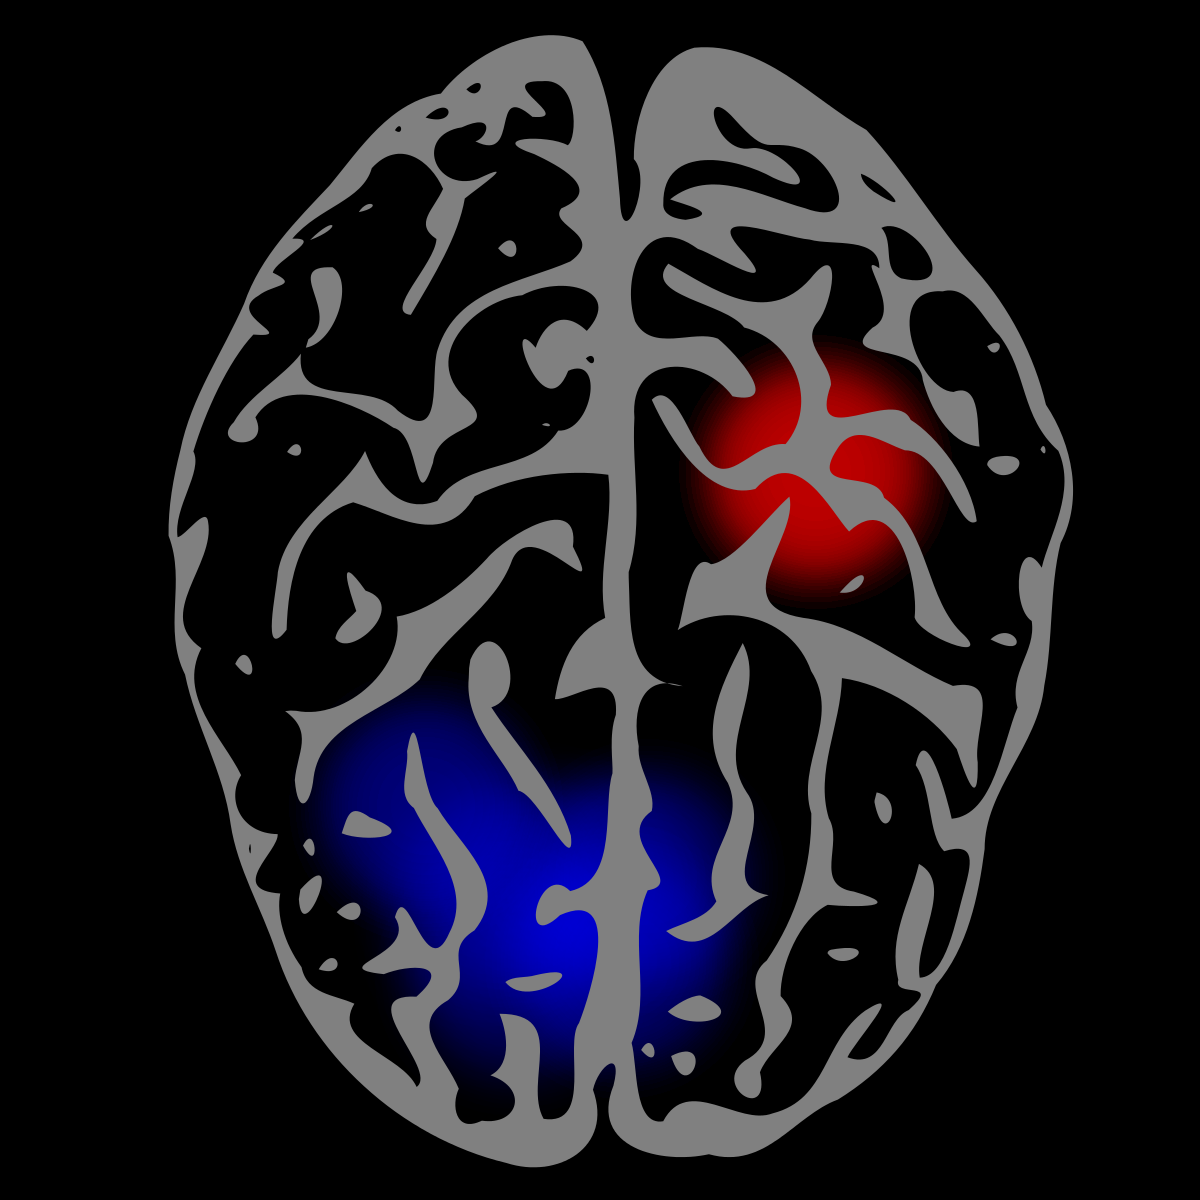
\includegraphics[scale = 0.07]{brain2.png} \\ \hline
\hspace{1in} & \hspace{1in} & \hspace{1in}
\end{tabular}
\end{center}
\end{frame}

\begin{frame}
\frametitle{Functional MRI}
\begin{center}
\begin{tabular}{ccc}
\hline
Stimuli $x$ & & Response $y$\\ \hline
$\begin{pmatrix}1.0 \\ 0 \\ 3.0 \\ 0\\ -1.2\end{pmatrix}$ & \hspace{1in} & $\begin{pmatrix}1.2 \\ 0 \\ -1.8\\ -1.2\end{pmatrix}$ \\ \hline
$\begin{pmatrix}0 \\ -2.2 \\ -3.1 \\ 4.5\\ 0\end{pmatrix}$ & \hspace{1in} & $\begin{pmatrix}-1.2 \\ -1.9\\ 0.5\\ 0.6\end{pmatrix}$ \\ \hline
\hspace{1in} & \hspace{1in} & \hspace{1in}
\end{tabular}
\end{center}
\end{frame}

\begin{frame}
\frametitle{Encoding vs Decoding}
\begin{itemize}
\item Encoding: predict $y$ from $x$.
\item Decoding: reconstruct $x$ from $y$ (mind-reading).
\end{itemize}
\end{frame}

\begin{frame}
\frametitle{A mind-reading game: Classification}
\begin{center}
Training Data
\\
\begin{tabular}{ccc||ccc}
\hline
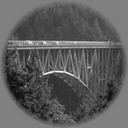
\includegraphics[scale = .26]{img1.png} & \hspace{0.2in} & 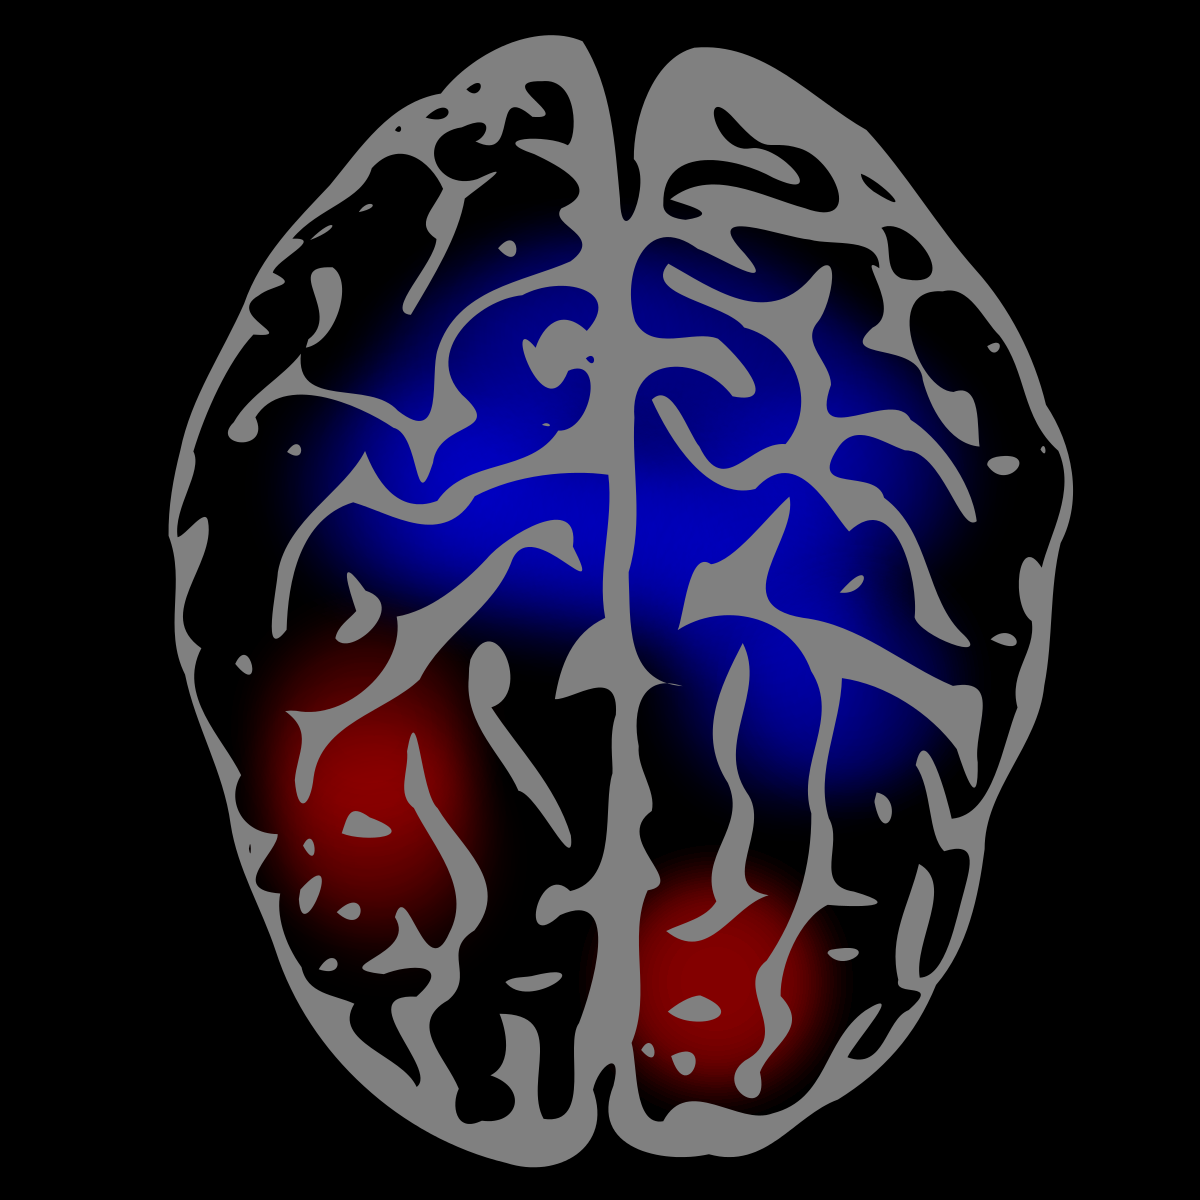
\includegraphics[scale = 0.035]{brain1.png} &
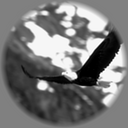
\includegraphics[scale = .26]{img3.png} & \hspace{0.2in} & 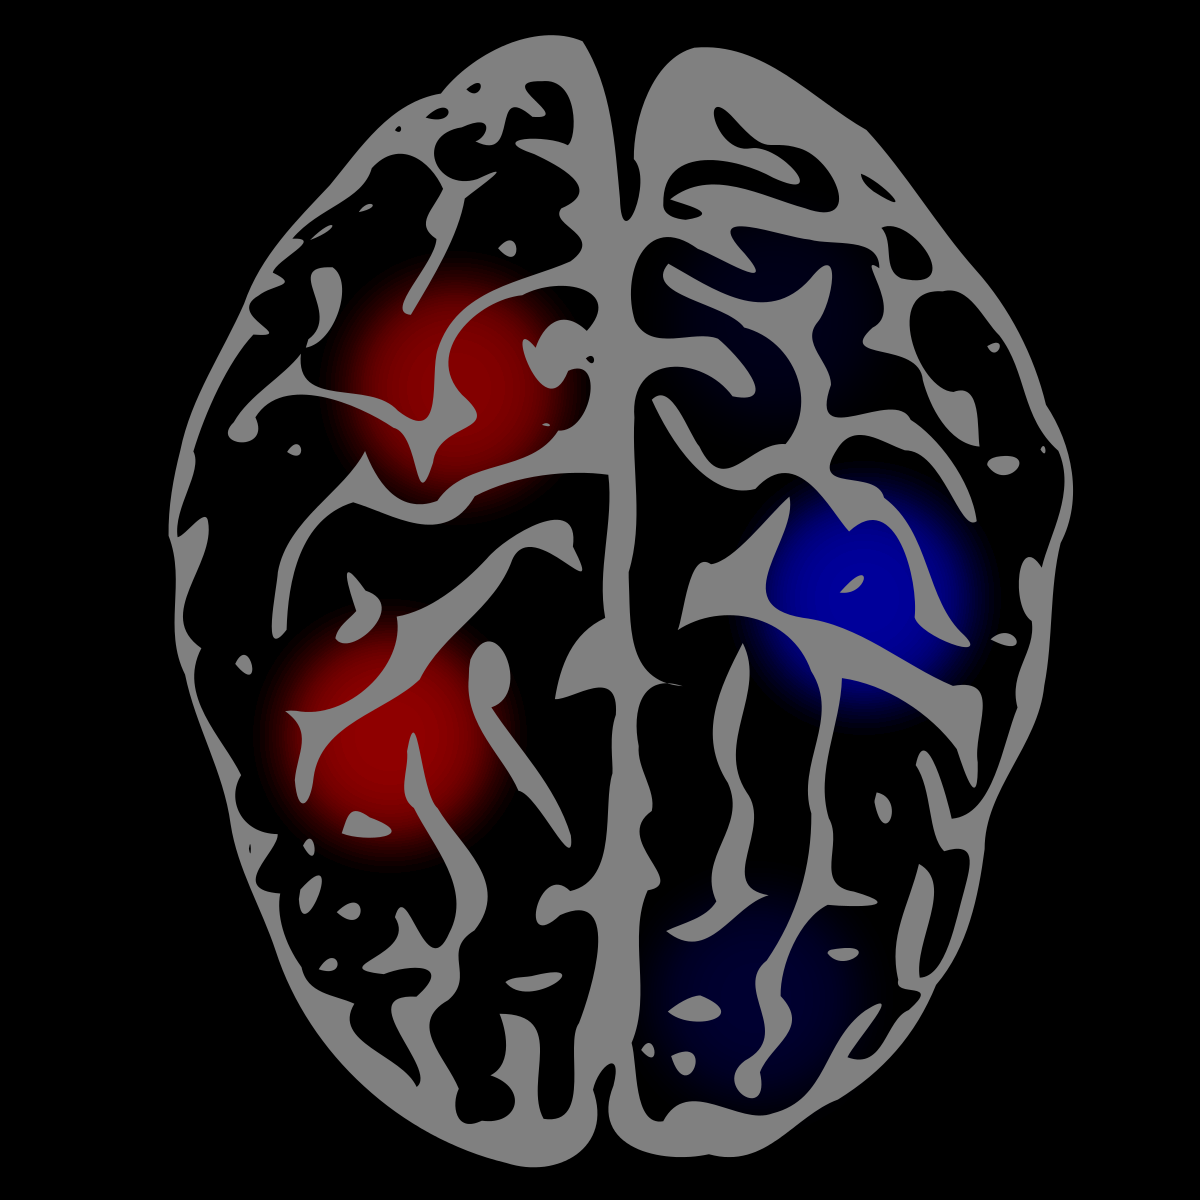
\includegraphics[scale = 0.035]{brain3.png} \\ \hline
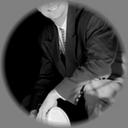
\includegraphics[scale = .26]{img2.png} & \hspace{0.2in} & 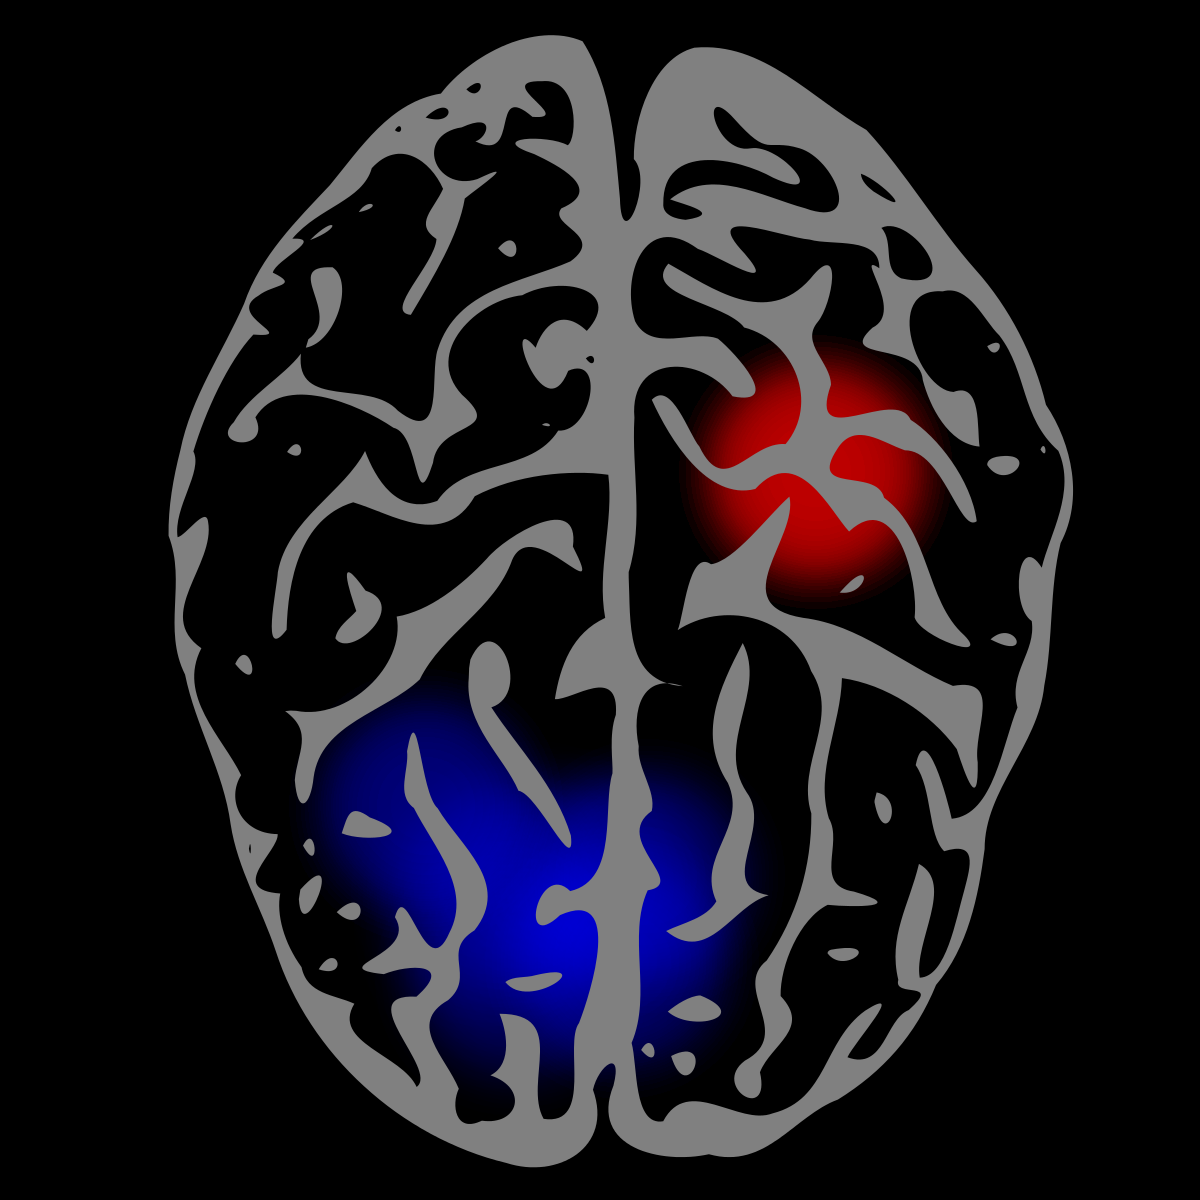
\includegraphics[scale = 0.035]{brain2.png} &
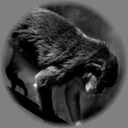
\includegraphics[scale = .26]{img4.png} & \hspace{0.2in} & 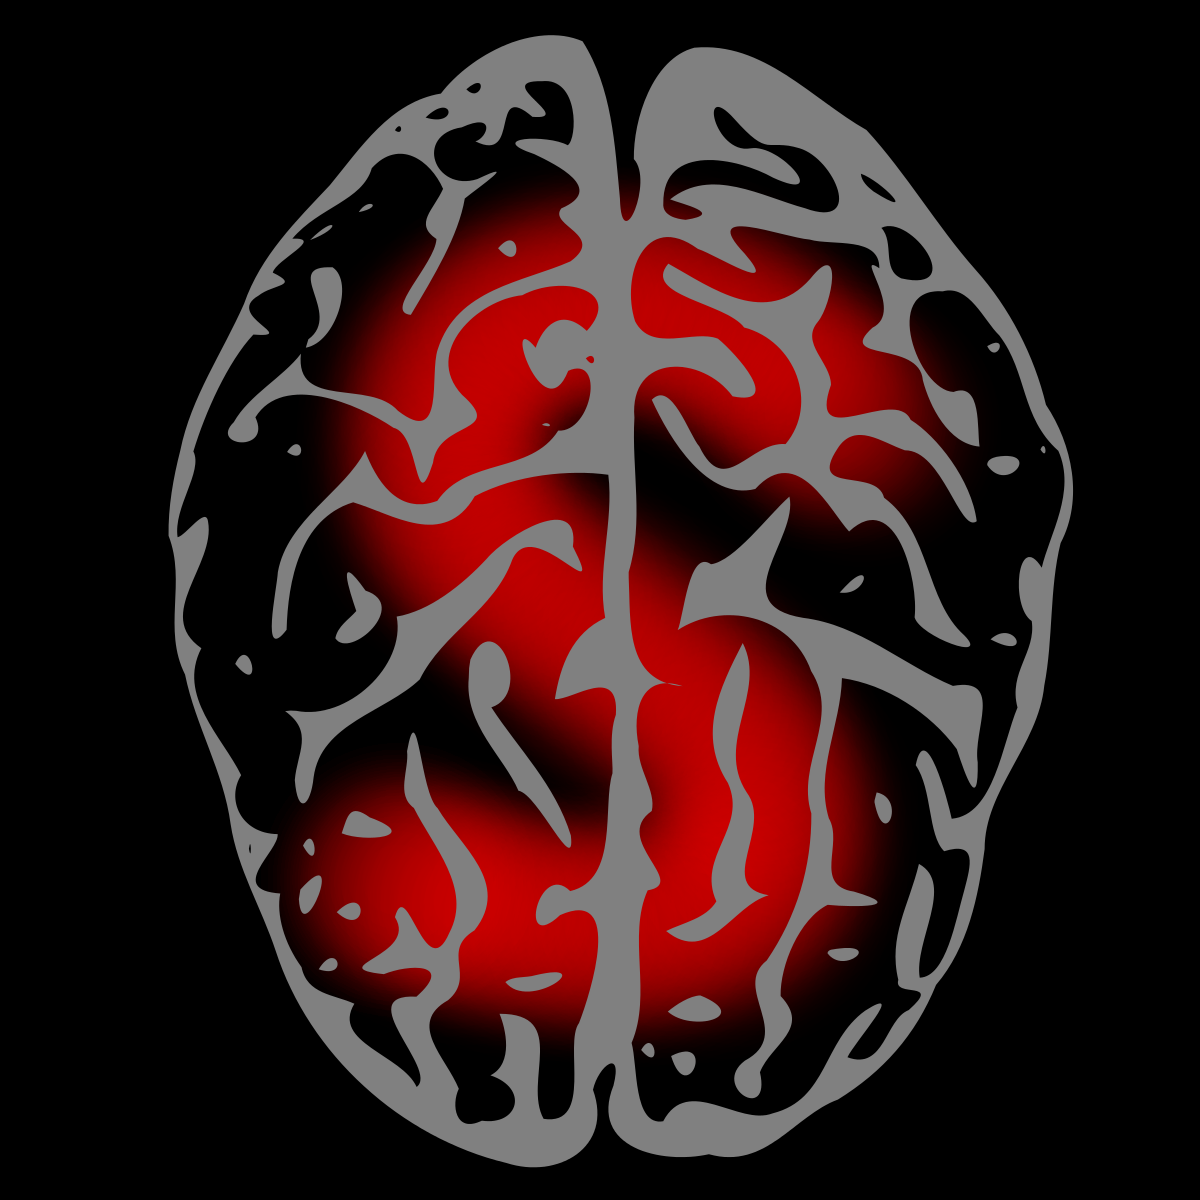
\includegraphics[scale = 0.035]{brain5.png} \\ \hline
\end{tabular}\\
\vspace{0.1in}
Test Data \\
\begin{tabular}{c|c|cccc}
\hline
 & & ? & ? & ? & ? \\
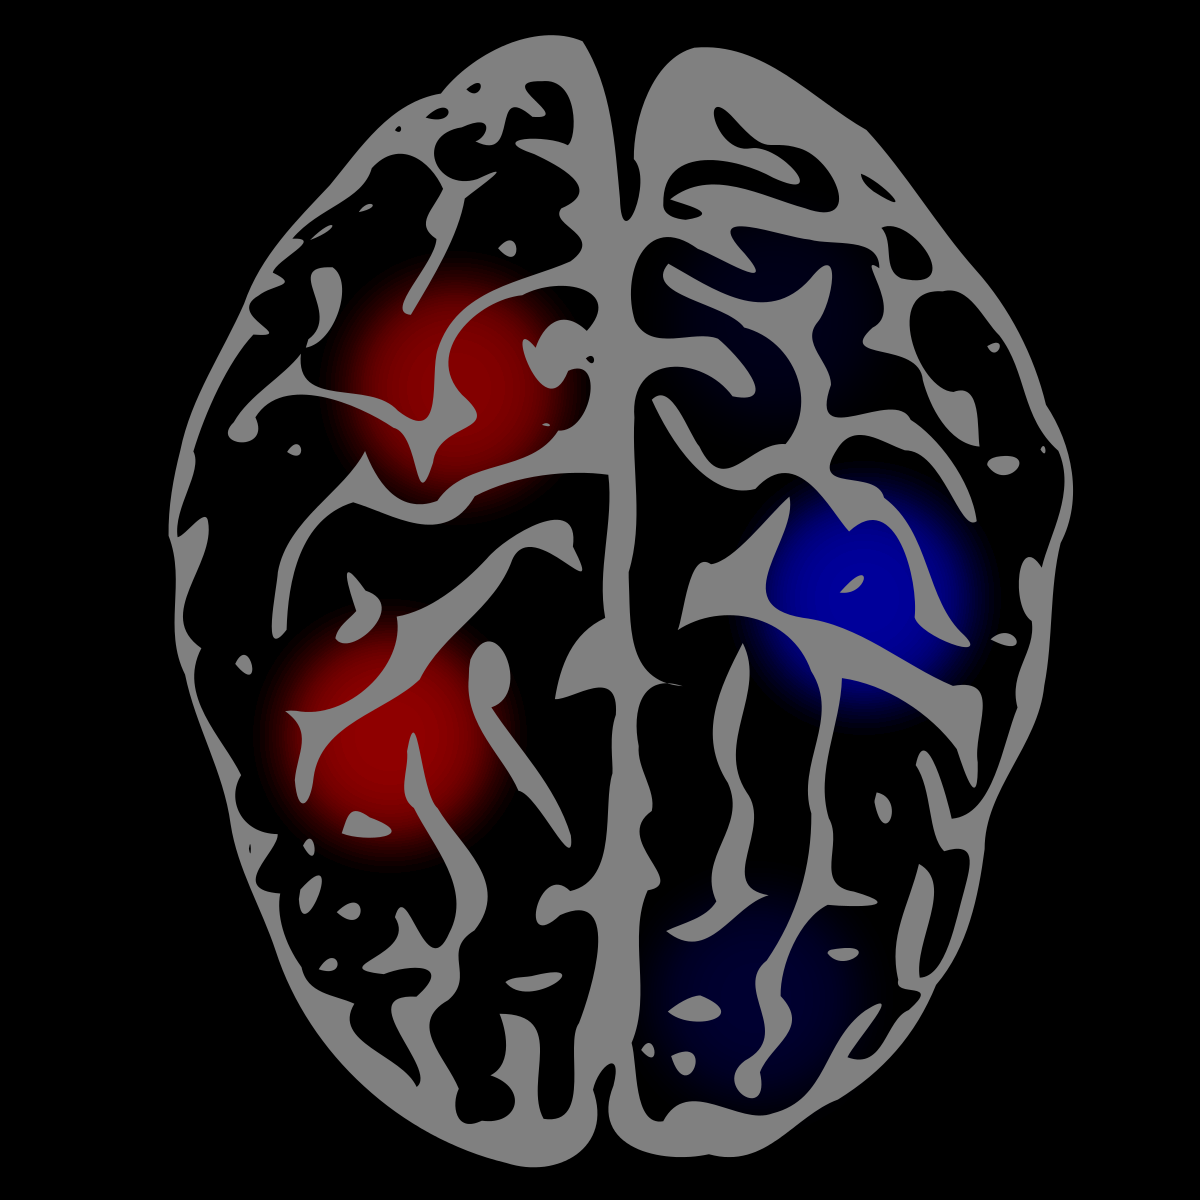
\includegraphics[scale = 0.035]{brain3.png} & \hspace{0.5in} 
& 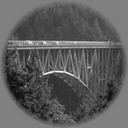
\includegraphics[scale = .26]{img1.png}
& 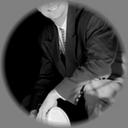
\includegraphics[scale = .26]{img2.png}
& 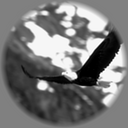
\includegraphics[scale = .26]{img3.png}
& 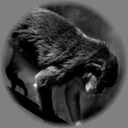
\includegraphics[scale = .26]{img4.png}\\
\hline
 & & ? & ? & ? & ? \\
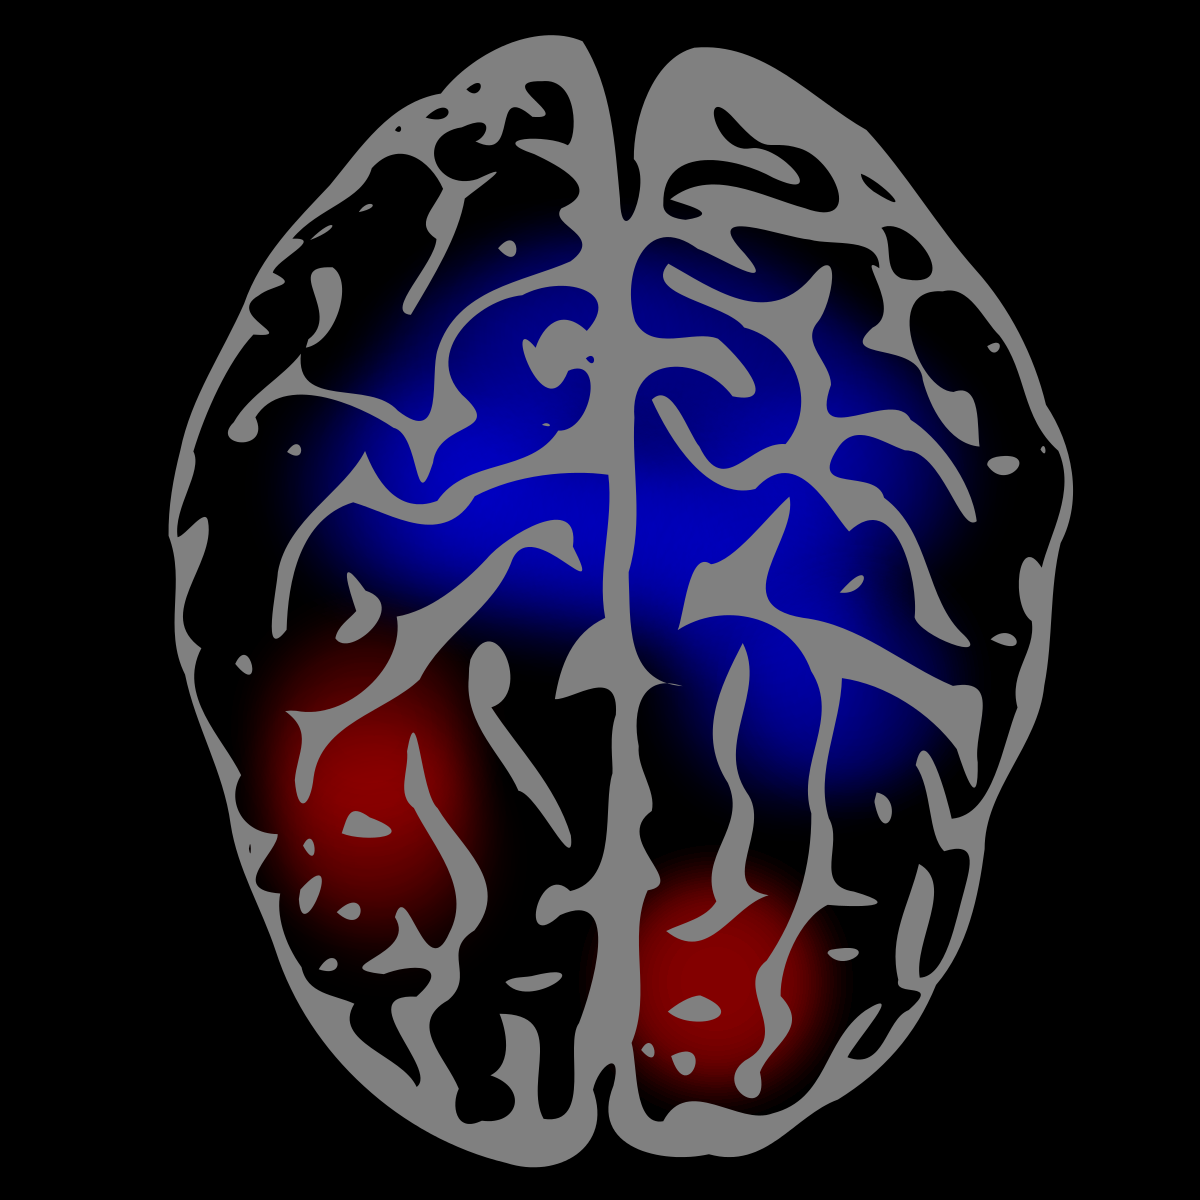
\includegraphics[scale = 0.035]{brain1.png} & \hspace{0.5in} 
& 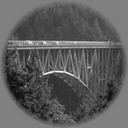
\includegraphics[scale = .26]{img1.png}
& 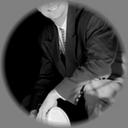
\includegraphics[scale = .26]{img2.png}
& 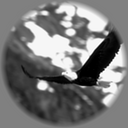
\includegraphics[scale = .26]{img3.png}
& 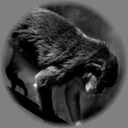
\includegraphics[scale = .26]{img4.png}\\
\hline
\end{tabular}
\end{center}
\end{frame}


\begin{frame}
\frametitle{A mind-reading game: Classification}
\begin{center}
Training Data
\\
\begin{tabular}{ccc||ccc}
\hline
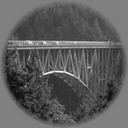
\includegraphics[scale = .26]{img1.png} & \hspace{0.2in} & 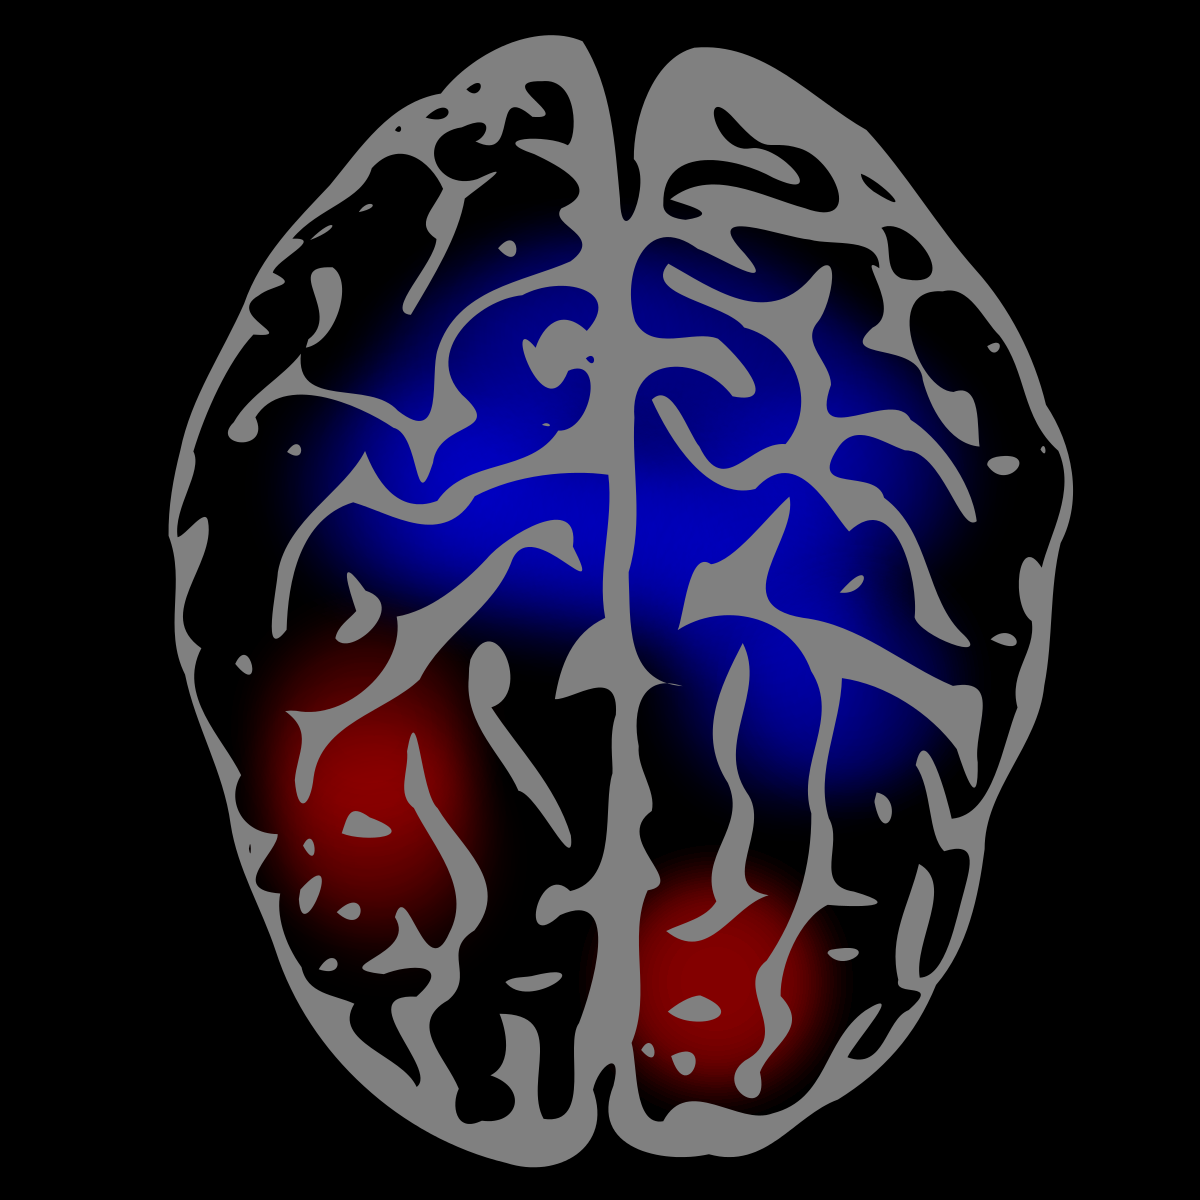
\includegraphics[scale = 0.035]{brain1.png} &
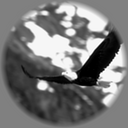
\includegraphics[scale = .26]{img3.png} & \hspace{0.2in} & 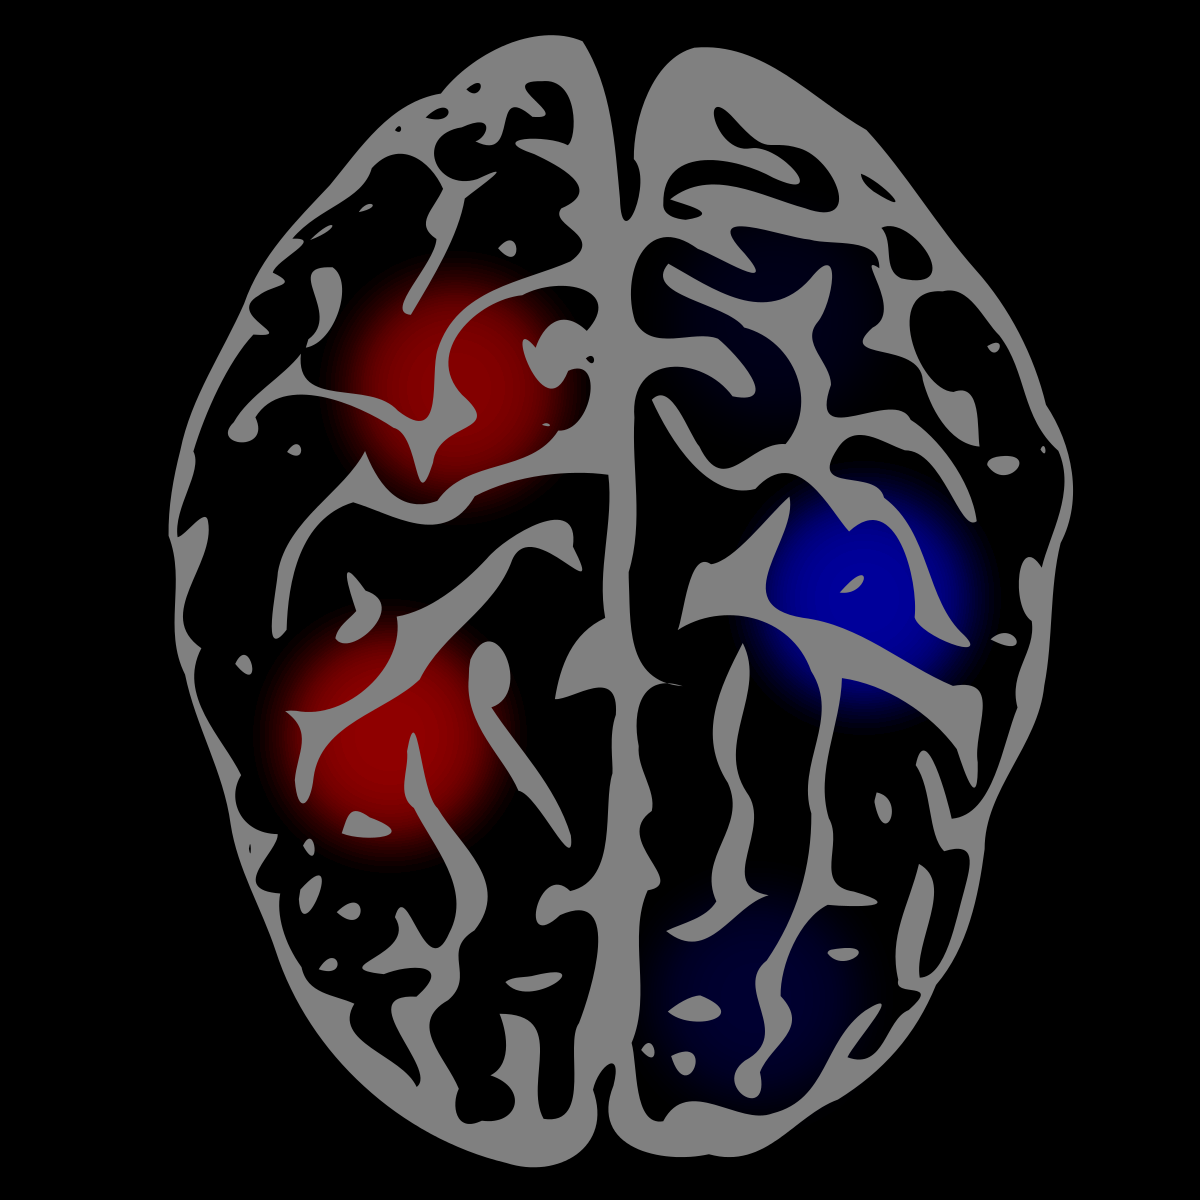
\includegraphics[scale = 0.035]{brain3.png} \\ \hline
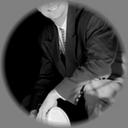
\includegraphics[scale = .26]{img2.png} & \hspace{0.2in} & 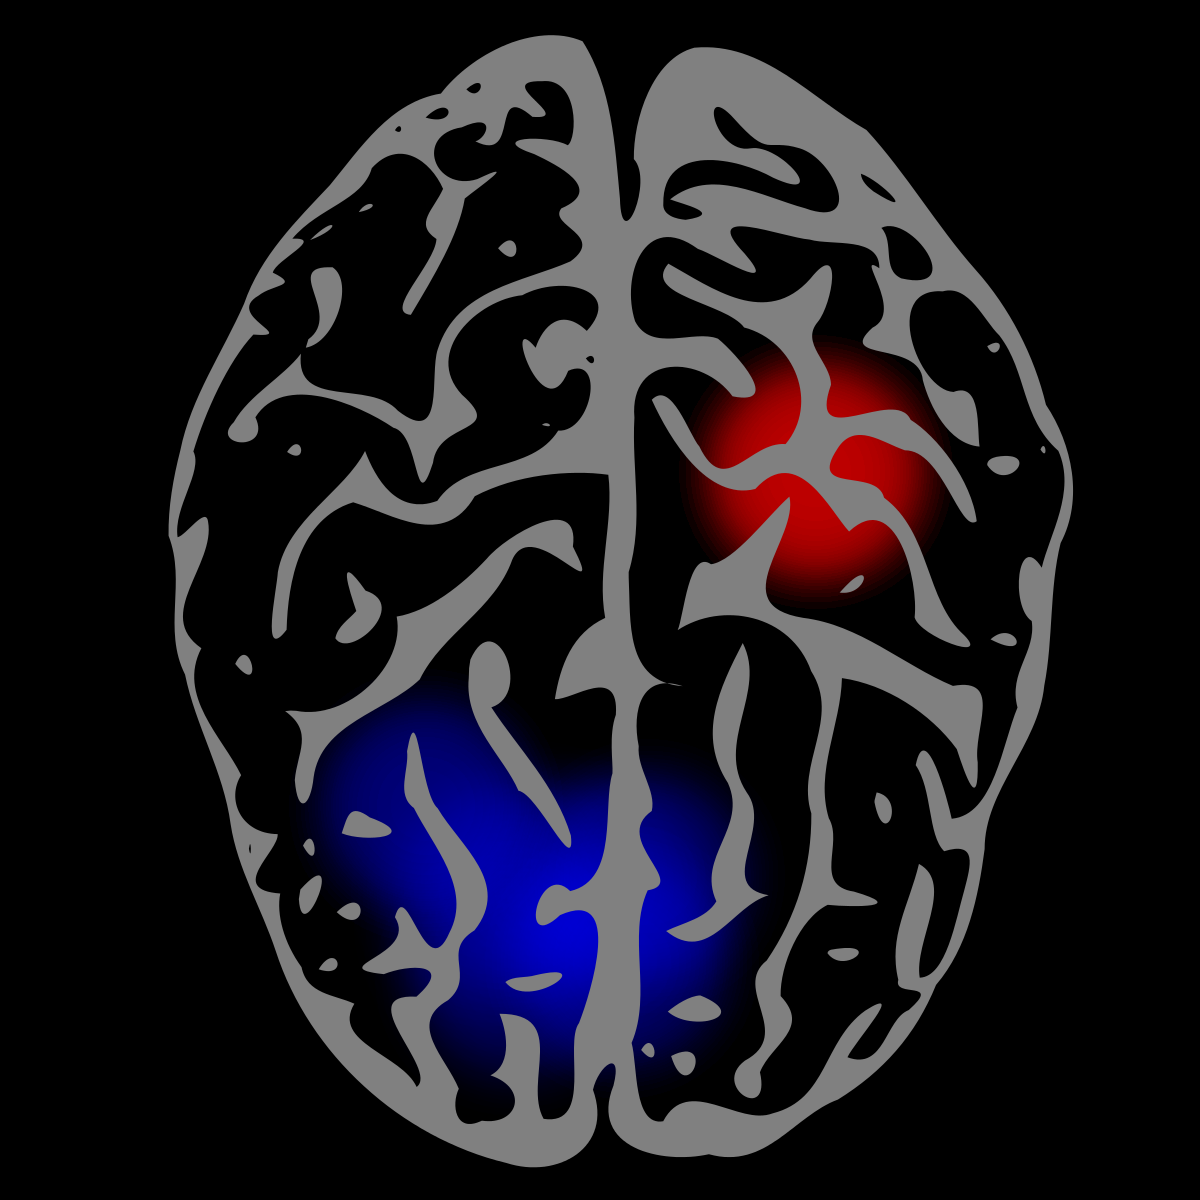
\includegraphics[scale = 0.035]{brain2.png} &
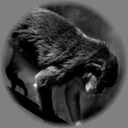
\includegraphics[scale = .26]{img4.png} & \hspace{0.2in} & 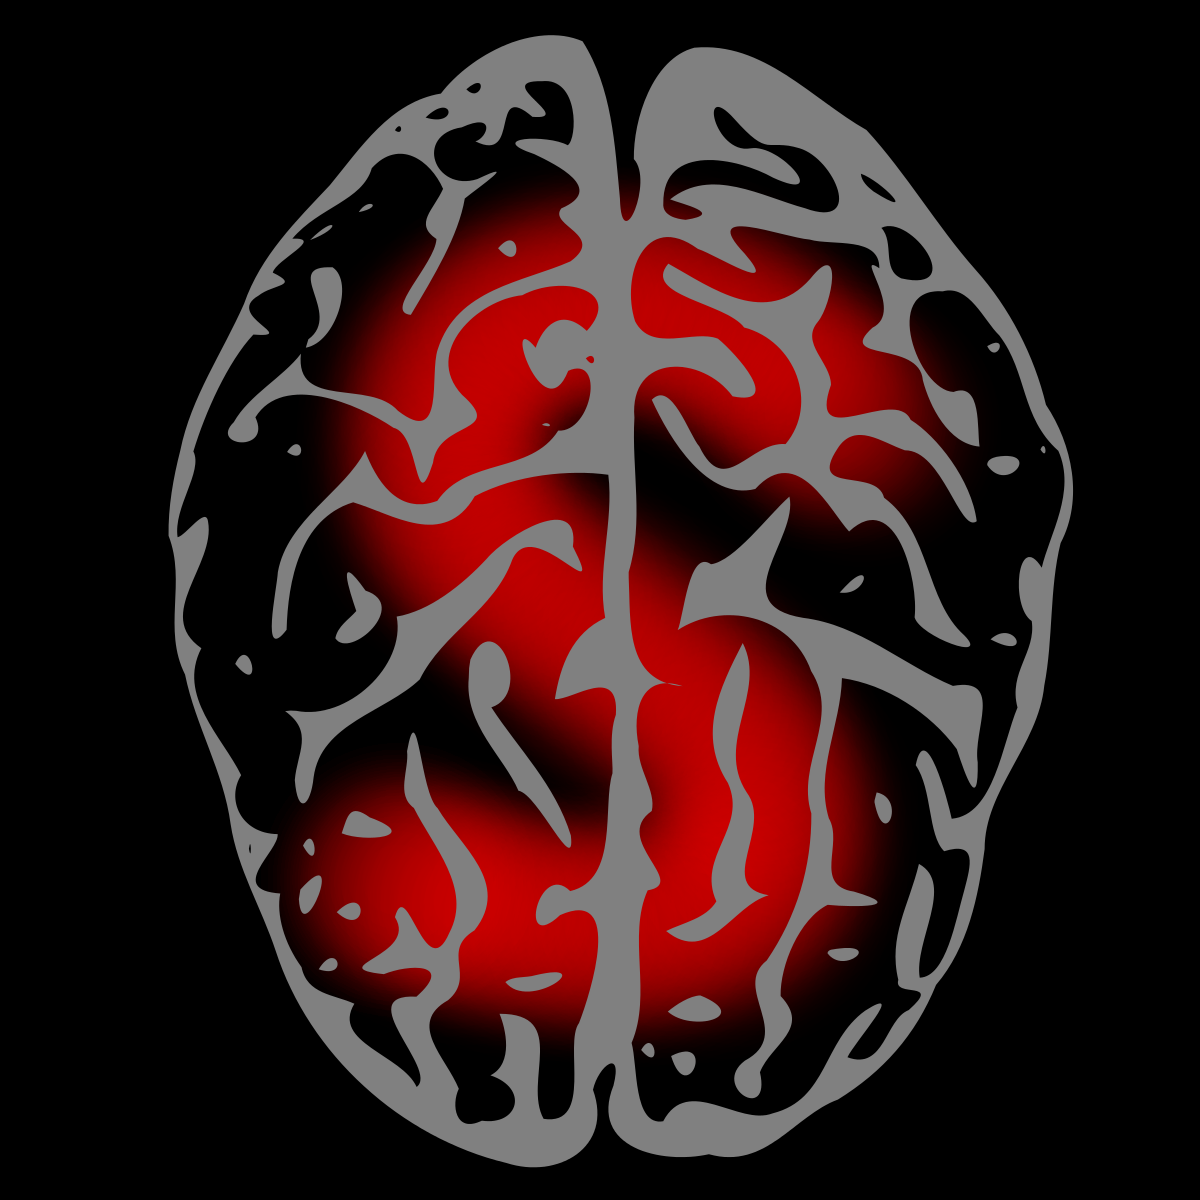
\includegraphics[scale = 0.035]{brain5.png} \\ \hline
\end{tabular}\\
\vspace{0.1in}
Test Data \\
\begin{tabular}{c|c|cccc}
\hline
 & & \xmark & \xmark & \cmark & \xmark \\
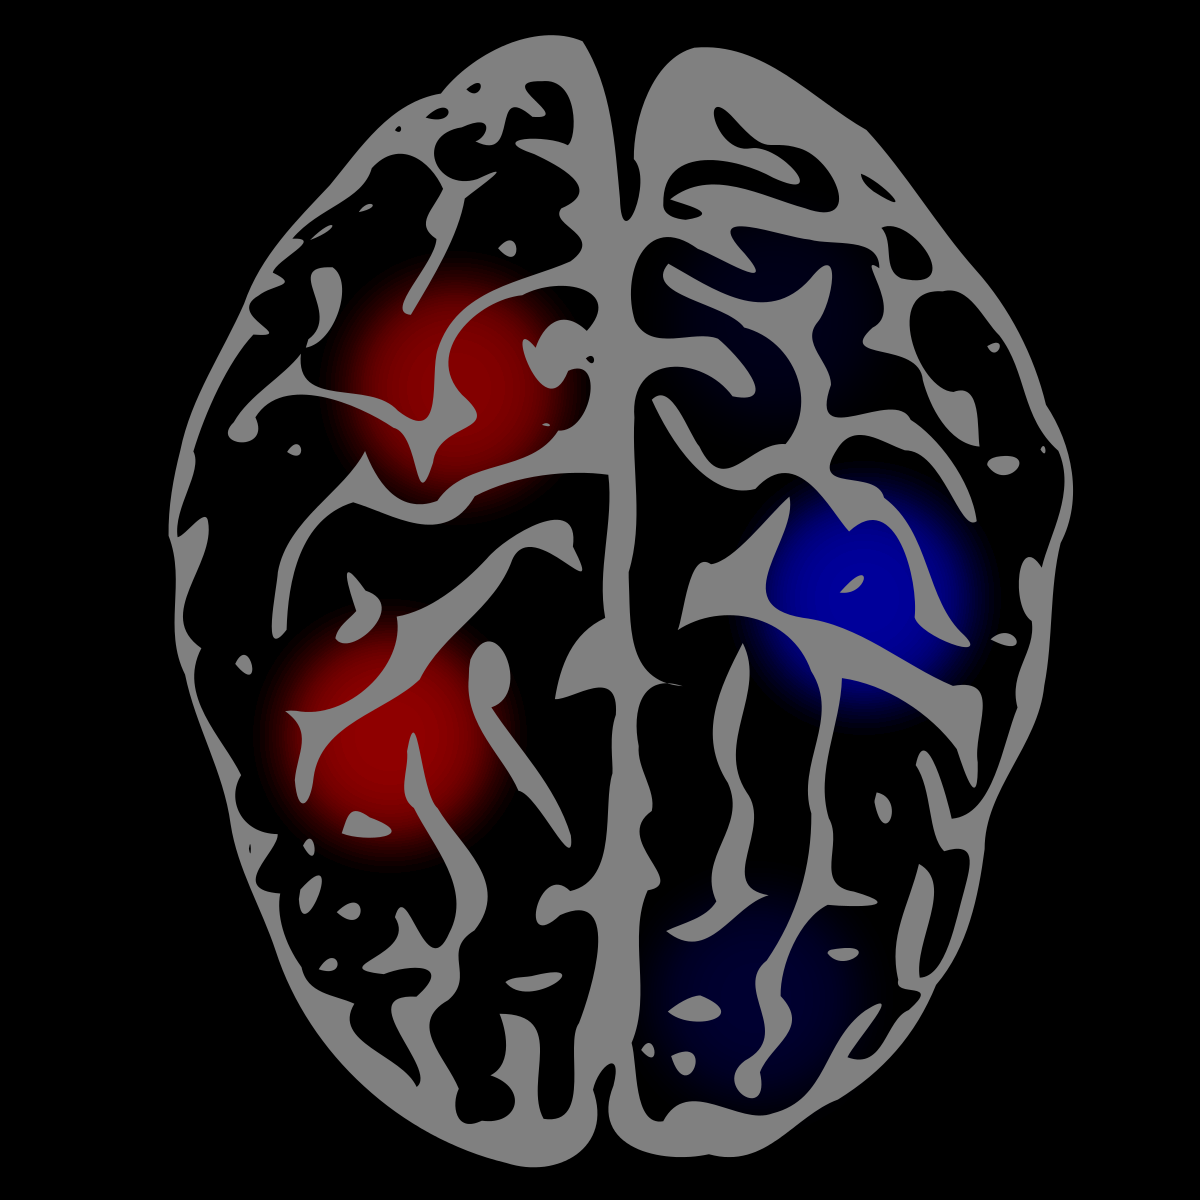
\includegraphics[scale = 0.035]{brain3.png} & \hspace{0.5in} 
& 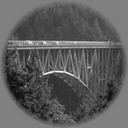
\includegraphics[scale = .26]{img1.png}
& 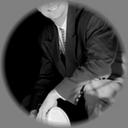
\includegraphics[scale = .26]{img2.png}
& 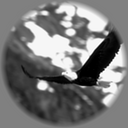
\includegraphics[scale = .26]{img3.png}
& 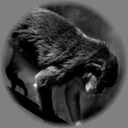
\includegraphics[scale = .26]{img4.png}\\
\hline
 & & \cmark & \xmark & \xmark & \xmark \\
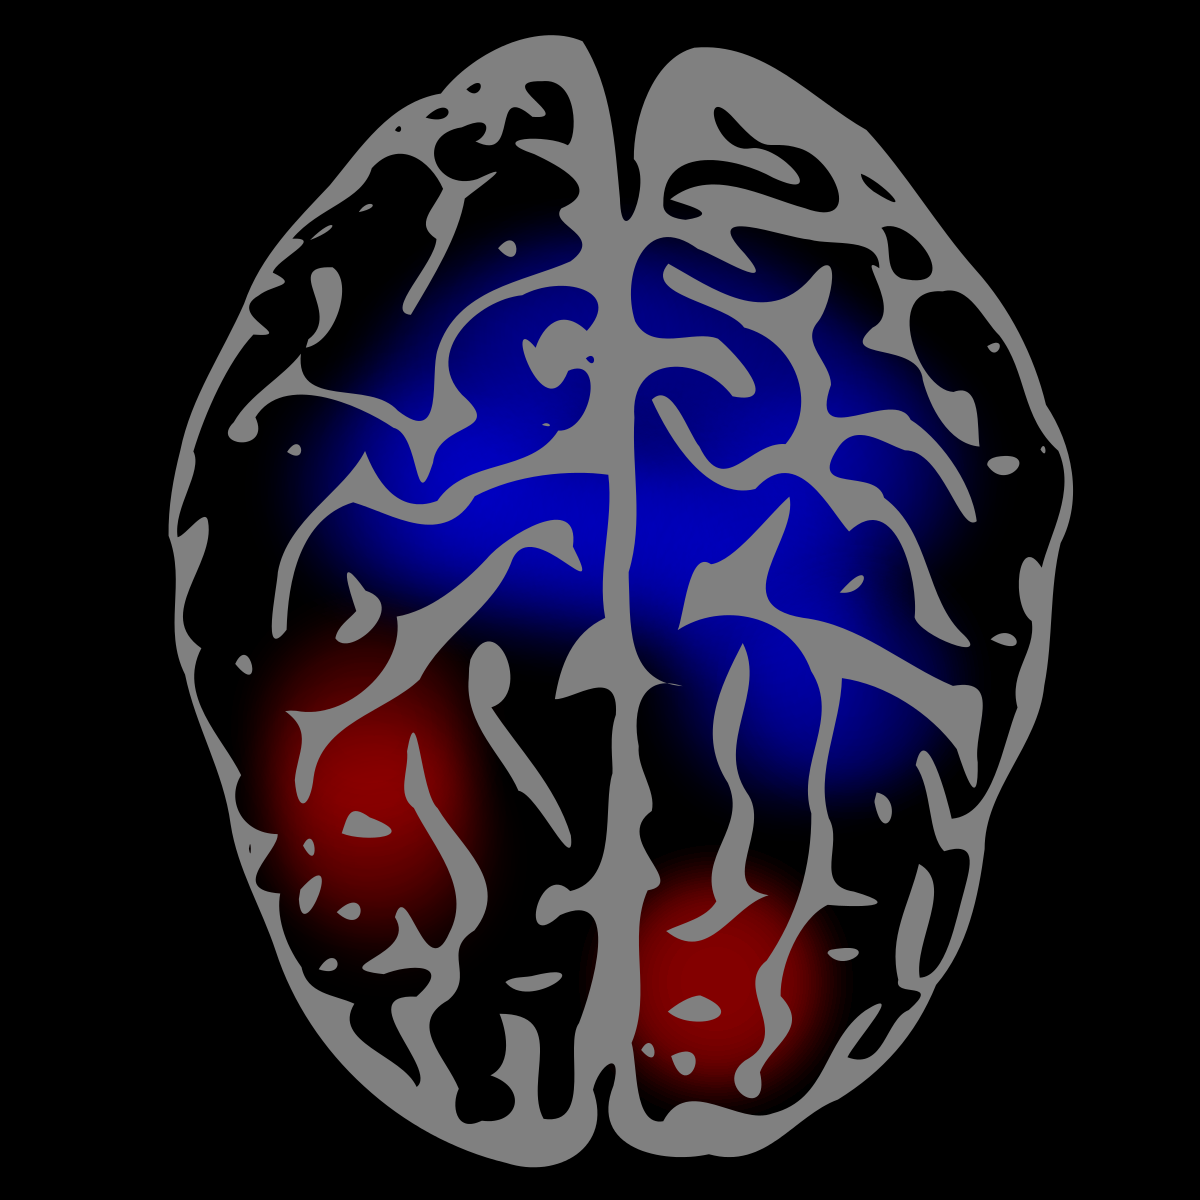
\includegraphics[scale = 0.035]{brain1.png} & \hspace{0.5in} 
& 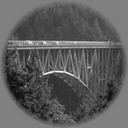
\includegraphics[scale = .26]{img1.png}
& 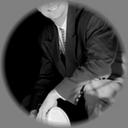
\includegraphics[scale = .26]{img2.png}
& 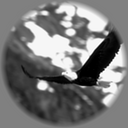
\includegraphics[scale = .26]{img3.png}
& 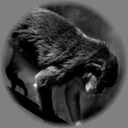
\includegraphics[scale = .26]{img4.png}\\
\hline
\end{tabular}
\end{center}
\end{frame}

\begin{frame}
\frametitle{A mind-reading game: Identification}
\begin{center}
Training Data
\\
\begin{tabular}{ccc||ccc}
\hline
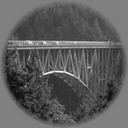
\includegraphics[scale = .26]{img1.png} & \hspace{0.2in} & 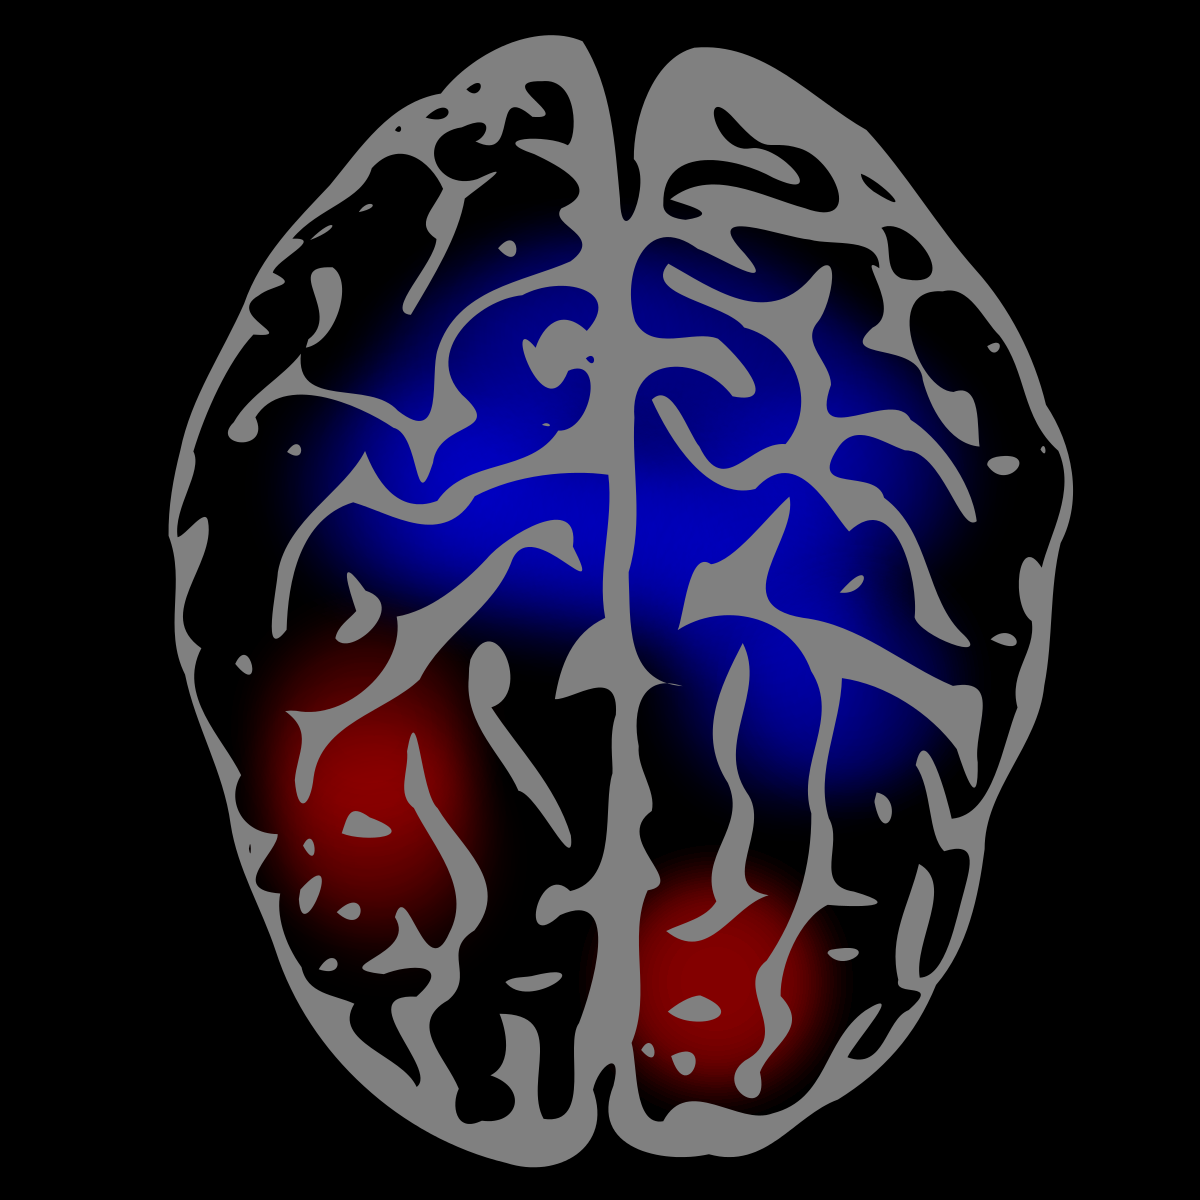
\includegraphics[scale = 0.035]{brain1.png} &
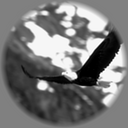
\includegraphics[scale = .26]{img3.png} & \hspace{0.2in} & 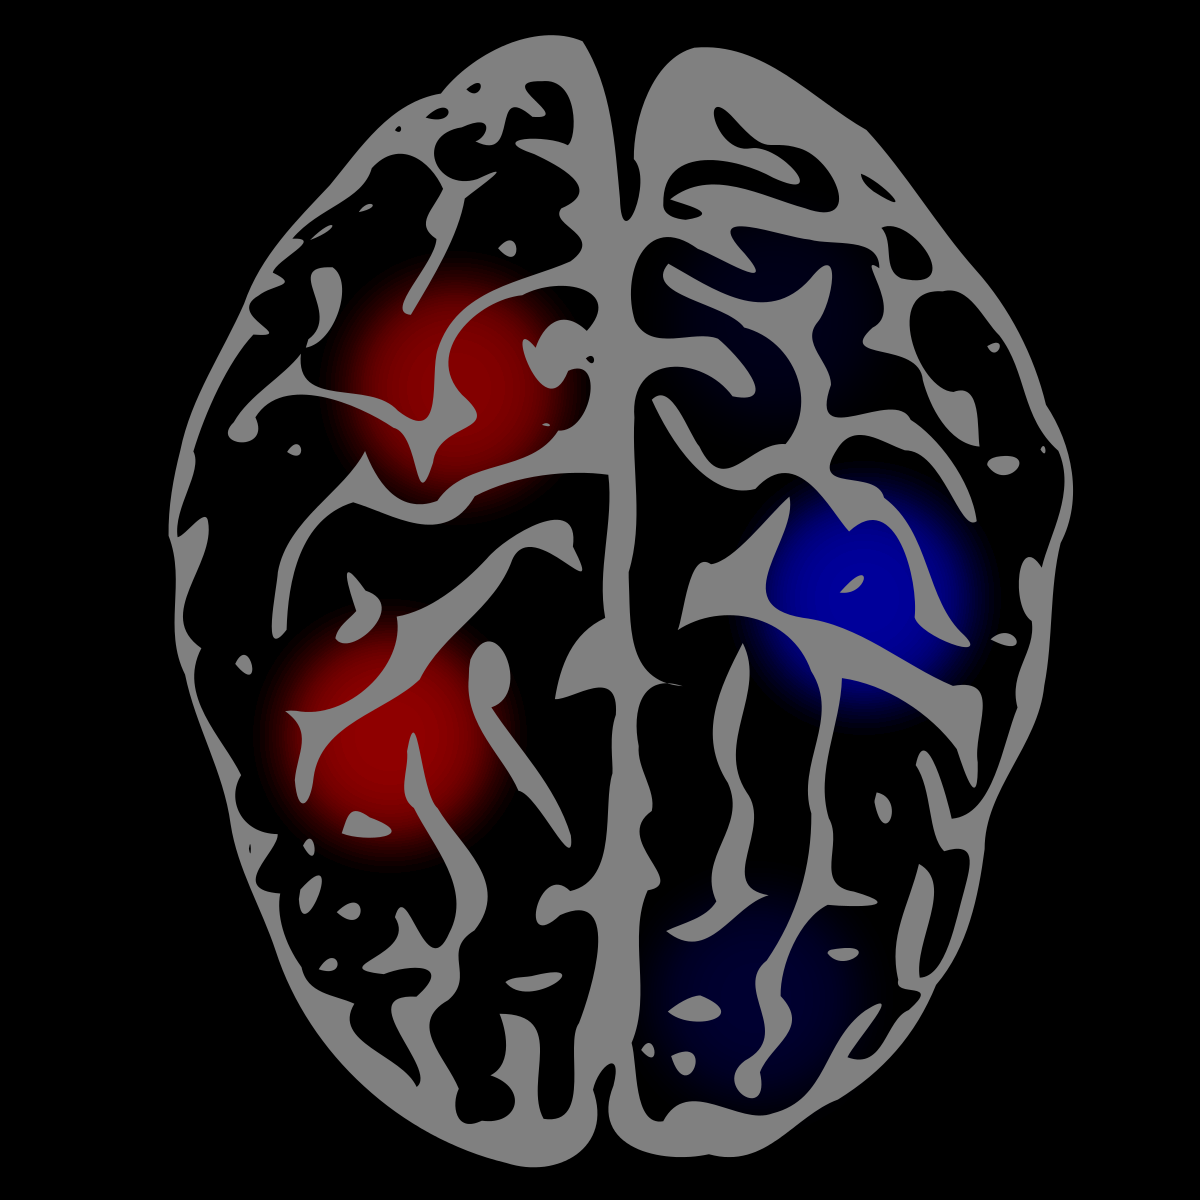
\includegraphics[scale = 0.035]{brain3.png} \\ \hline
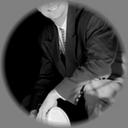
\includegraphics[scale = .26]{img2.png} & \hspace{0.2in} & 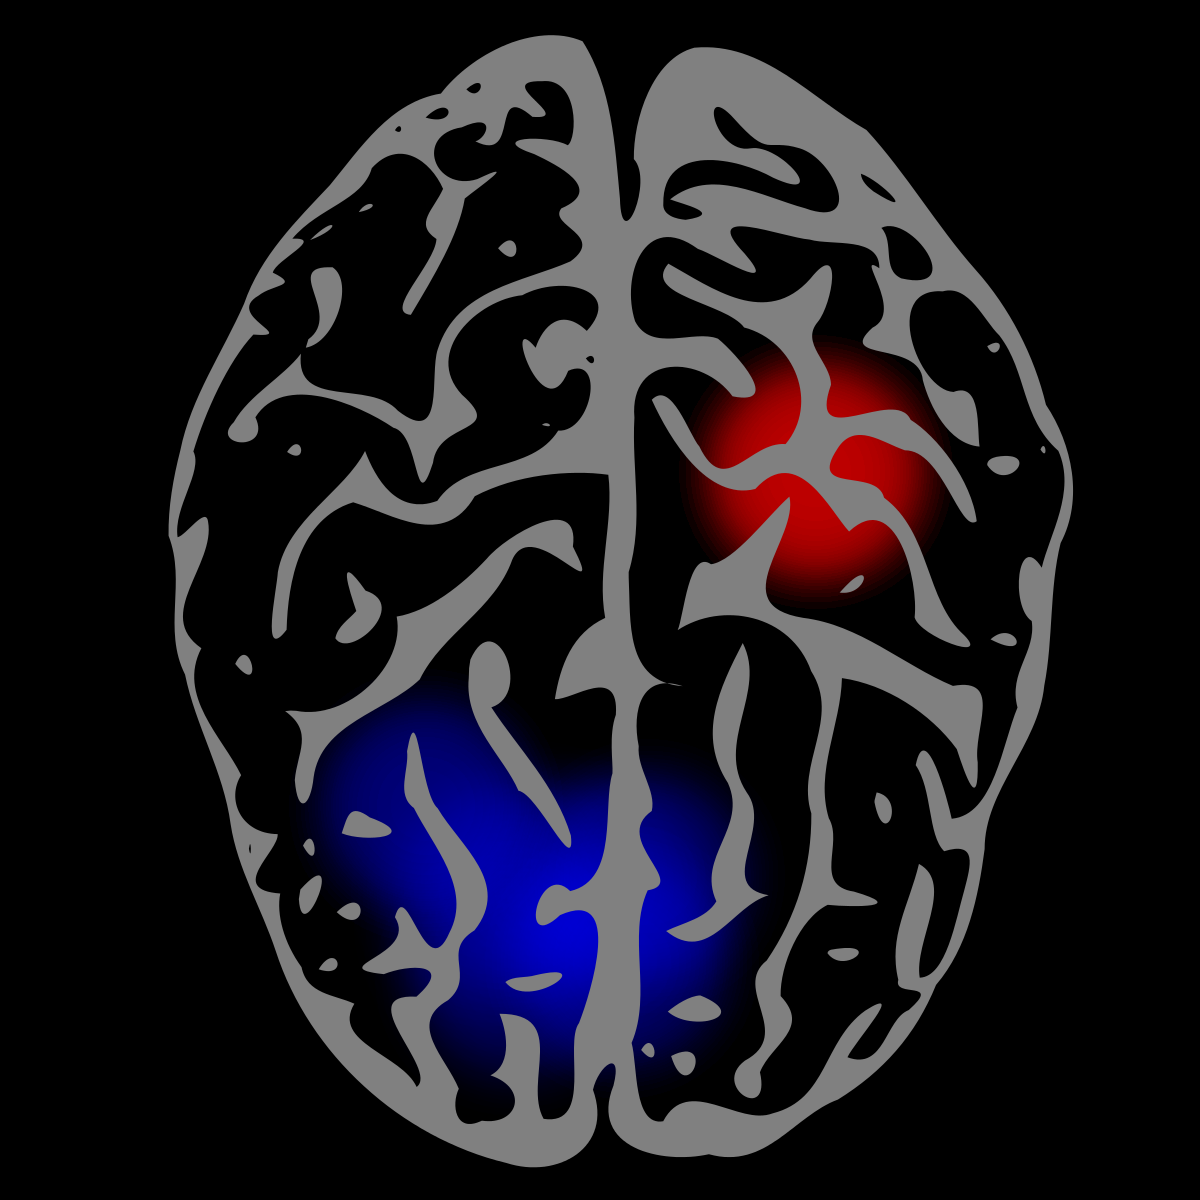
\includegraphics[scale = 0.035]{brain2.png} &
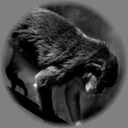
\includegraphics[scale = .26]{img4.png} & \hspace{0.2in} & 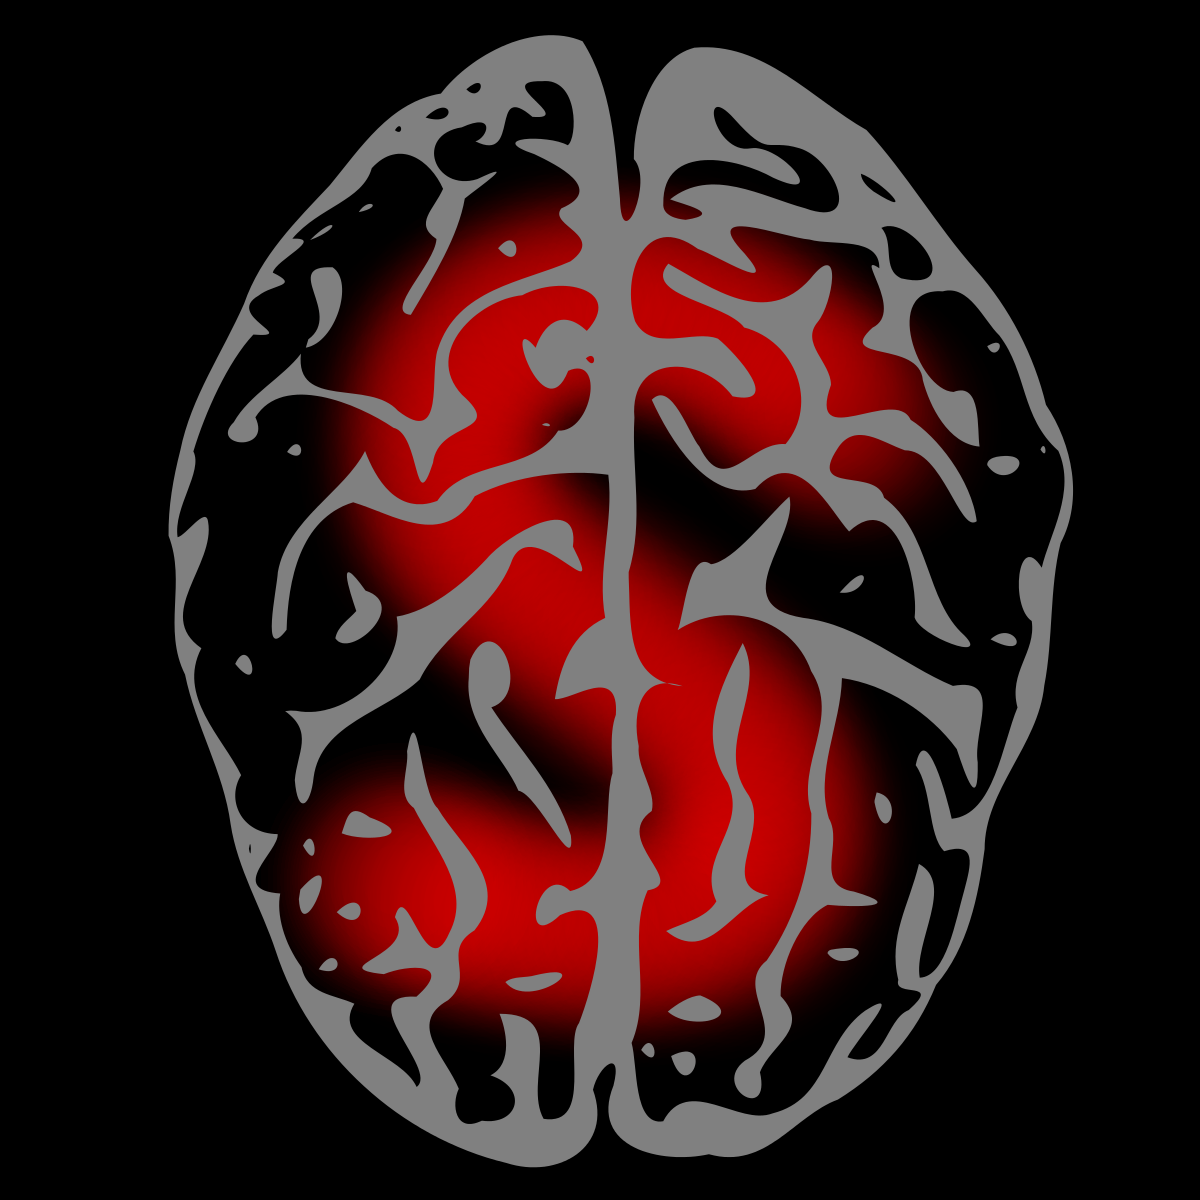
\includegraphics[scale = 0.035]{brain5.png} \\ \hline
\end{tabular}\\
\vspace{0.1in}
Test Data \emph{(new images!)} \\
\begin{tabular}{c|c|cccc}
\hline
 & & ? & ? & ? & ? \\
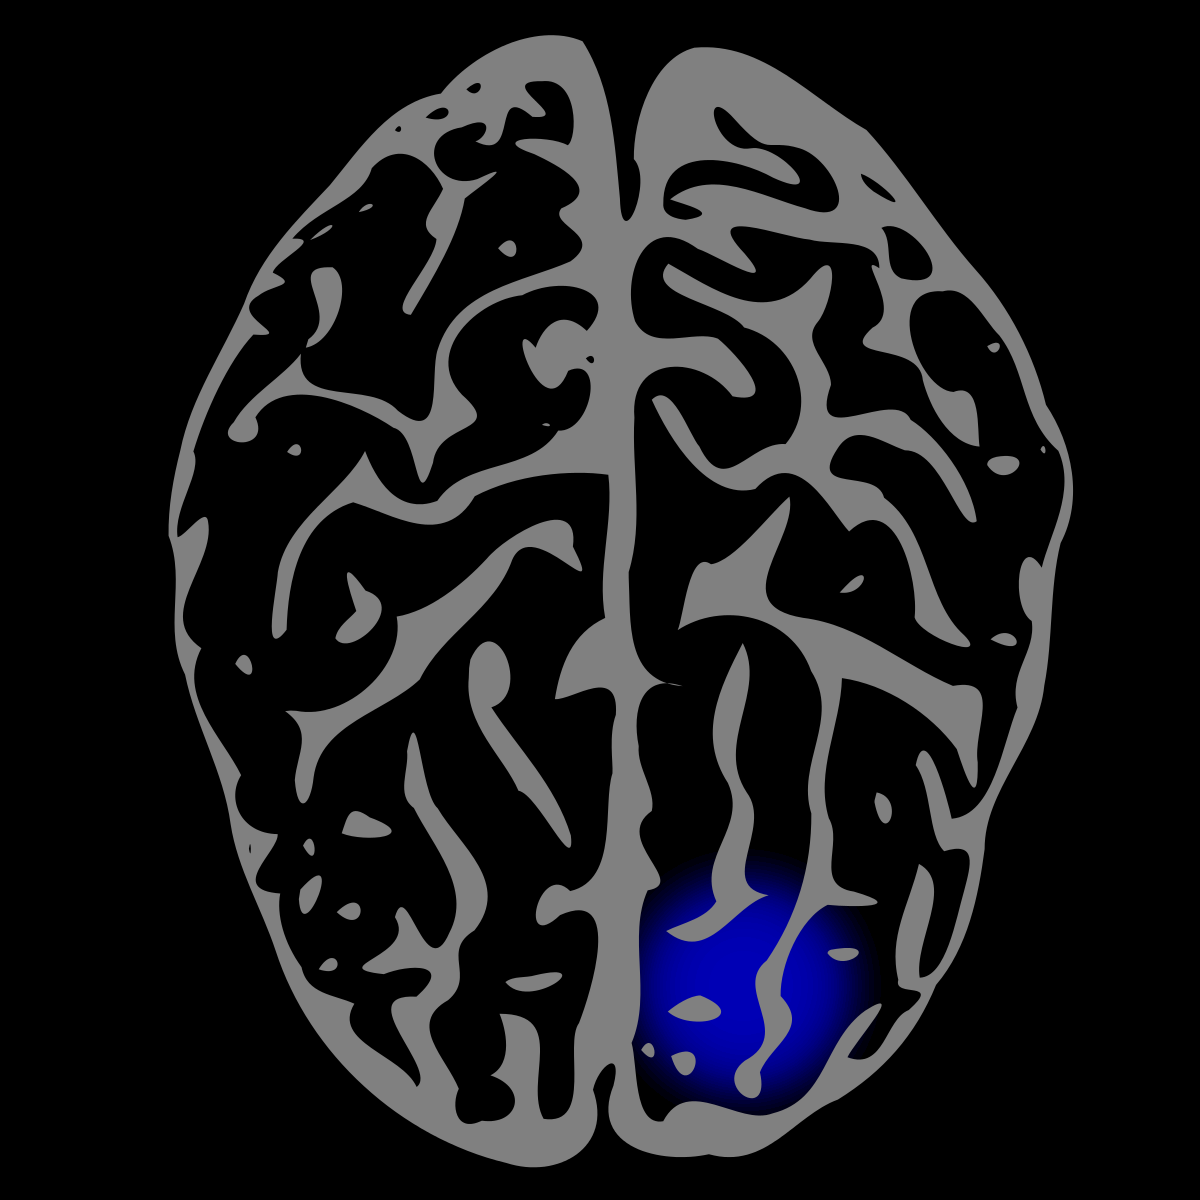
\includegraphics[scale = 0.035]{brain7.png} & \hspace{0.5in} 
& 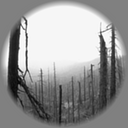
\includegraphics[scale = .26]{img5.png}
& \includegraphics[scale = .26]{img6.png}
& \includegraphics[scale = .26]{img7.png}
& \includegraphics[scale = .26]{img8.png}\\
\hline
 & & ? & ? & ? & ? \\
\includegraphics[scale = 0.035]{brain8.png} & \hspace{0.5in} 
& \includegraphics[scale = .26]{img5.png}
& \includegraphics[scale = .26]{img6.png}
& \includegraphics[scale = .26]{img7.png}
& \includegraphics[scale = .26]{img8.png}\\
\hline
\end{tabular}
\end{center}
\end{frame}

\begin{frame}
\frametitle{Statistical formulation I}
\emph{Training data.}
\begin{itemize}
\item
Given training classes $S_{\text{train}} = \{\text{train:}1,\hdots,
\text{train:}k\}$ where each class $\text{train:}i$ has features
$x_{\text{train:}i}$.
\item
For $t = 1,\hdots, T_{\text{train}}$, choose class label
$z_{\text{train:} t} \in S_{\text{train}}$; generate
\[
y_{\text{train:} t} = f(x_{z_{\text{train:} t}}) + \epsilon_t
\]
where $f$ is an unknown function, and $\epsilon_t$ is i.i.d. from a
known or unknown distribution.
\end{itemize}
\emph{Test data.}
\begin{itemize}
\item
Given test stimuli $S_{\text{test}} = \{\text{test:}1,\hdots,
\text{test:}\ell\}$ with features $\{x_{\text{test:} 1}, \hdots,
x_{\text{test:} \ell}\}$
\item
Task: for $t = 1,\hdots, T_{\text{test}}$, predict
$\hat{z}_{\text{test:} t} \in S_{\text{train}}$ from $y_{\text{test}:
  t}$; try to minimize misclassification rate
\end{itemize}
\end{frame}

\begin{frame}
\frametitle{Statistical formulation II}
\begin{itemize}
\item $f$ is an unknown function
\item $P$ is a known or unknown distribution over image features
\item \emph{Training data.} Draw $x_{\text{train:} i} \sim P$ for $i = 1\,hdots, k$.
\item \emph{Test data.} Draw $x_{\text{train:} i} \sim P$ for $i = 1\,hdots, \ell$.
\item Theoretical question: Analyze average misclassification rate when classes are generated this way
\end{itemize}
\end{frame}

\begin{frame}
\frametitle{Toy example I}
\emph{Model.}
\begin{itemize}
\item Features $x$ are one-dimensional real numbers, as are responses
  $y$.  Parameter $\beta$ is also a real number.
\item
Suppose we estimated $\hat{\beta}$ from training data.
\end{itemize}

\emph{Test data.}
\begin{itemize}
\item
Generate features $x_{\text{test:} 1}, \hdots,
x_{\text{test:} \ell}$ iid $N(0, \sigma^2_x)$.
\item
Hidden labels  $z_{\text{test:} t}$ are iid uniform from $S_{\text{train}}$.
Generate $y_{\text{test:} t} \sim N(\beta x_{z_{\text{test:} t}}, \sigma^2_\epsilon)$
\item
Estimate $\hat{z}_{\text{test:} t}$ by maximum likelihood assuming
$\hat{\beta}$ is correct.  Thus:
\[
\hat{z}_{\text{test:} t} = \text{argmin}_{z} (\hat{\beta} x_z -
y_{\text{test:} t})^2
\]
\end{itemize}
\end{frame}


\end{document}












